\documentclass[a4paper]{article}
\usepackage[14pt]{extsizes} % для того чтобы задать нестандартный 14-ый размер шрифта
\usepackage[utf8]{inputenc}
\usepackage[english, russian]{babel}
\usepackage{setspace,amsmath}
\usepackage{epigraph} % для эпиграфов и продвинутых цитат
\usepackage{csquotes} % ещё одна штука для цитат
\usepackage[unicode, pdftex]{hyperref} % подключаем hyperref (для ссылок внутри  pdf)
\usepackage{amssymb} % в том числе для красивого знака пустого множества
\usepackage{amsthm} % в т.ч. для оформления доказательств
\usepackage[left=20mm, top=15mm, right=15mm, bottom=15mm, footskip=7mm]{geometry} % настройки полей документа 
\usepackage[active]{srcltx}
\usepackage{indentfirst}
\usepackage{listings}
\usepackage{tocloft}
\usepackage{misccorr} 
\usepackage{graphicx}
\usepackage{caption}
\usepackage[style=numeric,sorting=none]{biblatex}
\DeclareCaptionLabelSeparator{defffis}{ --- }
\captionsetup{justification=centering,labelsep=defffis}
\graphicspath{{images/}}
\DeclareGraphicsExtensions{.jpg}
\renewcommand{\cftsecleader}{\cftdotfill{\cftsubsecdotsep}}
\newcommand{\ran}{{\rm ran}\,}
\newcommand{\diag}{{\rm diag}\,}
% переименовываем  список литературы в "список используемой литературы"
\addto\captionsrussian{\def\refname{Список используемой литературы}}
\addto\captionsrussian{\renewcommand\listfigurename{Список рисунков}}
\newcounter{totreferences}
\pretocmd{\bibitem}{\addtocounter{totreferences}{1}}{}{}
\newtheorem{theorem}{Теорема} % задаём выводимое слово (для теорем)
\newtheorem{definition}{Опредление} % задаём выводимое слово (для определений) 
% объявляем новые команды 
\newcommand{\RNumb}[1]{\uppercase\expandafter{\romannumeral #1\relax}}

\begin{document} % начало документа
\def\figurename{Рисунок}

\makeatletter
\lst@UserCommand\lstlistlistingname{Список листингов кода:}
\makeatother
 
% НАЧАЛО ТИТУЛЬНОГО ЛИСТА
\begin{center}
\textbf{Министерство науки и высшего образования Российской Федерации}
\footnotesize{\textbf{ФЕДЕРАЛЬНОЕ ГОСУДАРСТВЕННОЕ АВТОНОМНОЕ ОБРАЗОВАТЕЛЬНОЕ УЧРЕЖДЕНИЕ ВЫСШЕГО ОБРАЗОВАНИЯ}}

\small{\textbf{<<НАЦИОНАЛЬНЫЙ ИССЛЕДОВАТЕЛЬСКИЙ УНИВЕРСИТЕТ ИТМО>>
(УНИВЕРСИТЕТ ИТМО)}}\\
\hfill \break
\small{\textbf{ЦЕНТР АВТОРИЗОВАННОГО ОБУЧЕНИЯ ИНФОРМАЦИОННЫМ
ТЕХНОЛОГИЯМ}}\\
 \hfill \break
\hfill\break
\hfill\break
\hfill \break
\hfill \break
\hfill \break
\large{\textbf{ДИПЛОМНАЯ РАБОТА}}\\
\hfill \break
\hfill \break
\large{\textbf{Разработка веб-приложения с
использованием\newline Spring Framework}\\
\hfill \break
\hfill \break
\hfill \break}
\end{center}

\normalsize{ 
\begin{tabular}{lllc}
\textbf{Автор} & $\underset{\text{(Подпись)}}{\underline{\hspace{5 cm}}}$ &  Нежберт К.Э.\\\\
\textbf{Специализация} & \underline{\hspace{0.3 cm}<<Java-разработчик>>\hspace{0.3 cm}}  \\\\
\textbf{Руководитель} & $\underset{\text{(Подпись)}}{\underline{\hspace{5 cm}}}$ &  Петров Р.А. \\\\
\textbf{К защите допустить} \\\\
\textbf{Руководитель ОП} & $\underset{\text{(Подпись)}}{\underline{\hspace{5 cm}}}$ &  Зудилова Т.В.
\end{tabular}
}\\
\hfill \break
\begin{flushright}
<<\underline{\hspace{1.5 cm}}>>\underline{\hspace{5 cm}} 2020 г.
\end{flushright}
\hfill \break
\begin{center} Санкт-Петербург, 2020 \end{center}
\thispagestyle{empty} % выключаем отображение номера для этой страницы

\newpage
\thispagestyle{empty}

Слушатель $\underset{\text{(ФИО}}{\underline{\hspace{7 cm}}}$ \hspace{4 cm} Группа \underline{\hspace{0.3 cm}124/6\hspace{0.3 cm}}
\newline

Специализация \underline{\hspace{0.3 cm}<<Java-разработчик>>\hspace{0.3 cm}}
\newline

Дипломная работа принята <<\underline{\hspace{1.5 cm}}>>\underline{\hspace{5 cm}} 2020 г.
\newline

Дипломная работа выполнена с оценкой \underline{\hspace{7 cm}}
\newline

Дата защиты <<\underline{\hspace{1.5 cm}}>>\underline{\hspace{5 cm}} 2020 г.
\newline

Секретарь $\underset{\text{(ФИО}}{\underline{\hspace{7 cm}}}$ \hspace{1 cm}  $\underset{\text{(Подпись}}{\underline{\hspace{5 cm}}}$
\newline

Листов хранения \underline{\hspace{7 cm}}
\newline

Демонстрационных материалов/чертежей хранения \underline{\hspace{5 cm}}
\newline
 
% КОНЕЦ ТИТУЛЬНОГО ЛИСТА
 
\newpage 
	\addcontentsline{toc}{section}{Содержание} 
    \tableofcontents % Вывод содержания
\newpage

\section{Используемые сокращения}


\textbf{CRUD} – Сreate, Read, Update, Delete

\textbf{CSS} – Cascading Style Sheets

\textbf{DDL} – Data Description Language

\textbf{DI} – Dependency Injection

\textbf{HTML} – HyperText Markup Language

\textbf{IoC} – Inversion of Control

\textbf{JDBC} – Java Database Connectivity

\textbf{JPA} – Java Persistence API

\textbf{JS} – JavaScript

\textbf{MVC} – Model-View-Controller

\textbf{ORM} – Object-Relational Mapping

\textbf{БД} – База данных

\textbf{СУБД} – система управления базами данных

\newpage

\section{Введение}

Пояснительная записка содержит: 30 стр., 19 рис., 11 листингов кода, 4 источника
литературы. 

В данной работе представлен обзор используемого стека технологий (языков и
фреймворков), представлено описание этапов процесса разработки, начиная с
анализа предметной области, определения сущностей предметной области, разработки базы
данных и интерфейса пользователя, а так же приведен обзор логики серверной и клиентской
частей приложения.

\subsection{Цель работы}
Цель работы: разработка веб-приложения на языке Java с использованием фреймворков Spring Framework и Hibernate под конкретную задачу.

\subsection{Описание задачи}
Основной задачей разрабатываемого приложения является осуществление коммуникации между сотрудниками предприятия и дирекцией корпоративной столовой этого же предприятия. На текущий момент на предприятии прекращено самостоятельное приготовление пищи и осуществлен переход на закупку готовых комплексов обедов в сторонней фирме. 

Для оптимизации расходов предприятия руководством была поставлена задача организовать удобный обмен данными между сотрудниками, обедающими в столовой, и дирекцией последней с целью конкретизации списка требуемых комплексов на каждый конкретный день.

\subsection{Выполненные работы}

В ходе выполнения данной дипломной работы выполнены следующие работы:
\begin{itemize}
\setlength{\itemsep}{-2mm}
	\item проведен сбор информации с непосредственного заказчика - директора столовой предприятия
	\item разработано клиент-серверное веб-приложение: <<Corporate Food Checker>>
	\item изучены технологии создания веб-приложений с использованием Spring Framework
(web, data-jpa, security) – наиболее широко распространенная технология разработки веб-
приложений для языка Java;
	\item изучены технологии представления данных для браузера (шаблонизатор html-страниц
Freemaker)
	\item изучены возможности свободного фреймворка для создания сайтов и веб-приложений BootStrap
	\item создана база данных на основе СУБД MySQL 
	\item изучены возможности системы контроля версий Git (код проекта лежит в закрытой репозитории хранилища кода GitHub, доступ к нему открыт только дипломному руководителю с самого начала разработки).
	\item изучены возможности системы сборки Maven
\end{itemize}

Результаты данной дипломной работы будут использоваться в реальной компании - заводе по производству молочной продукции в Ленинградской Области. Также предусмотрен задел на будущее - широкое поле для доработок и улучшений, предусматривающих также более глубокое изучение представленного выше стека технологий.

\section{Цели и задачи}
Для реализации основной цели данной дипломной работы необходимо привести краткий обзор бизнес-проблемы.

\subsection{Краткий обзор ситуации}
На текущий момент решения задачи как такового не было. Были попытки организовать сообщение между работниками и сотрудниками столовой посредством телефона (звонок на определенный номер и сообщения своего выбора), а также непосредственный физческий контакт в виде обхода всех отделов с физическим носитилем (блокнотом) и последующим ручным подбиванием полученных данных.

Такие методы не оправдывают себя по нескольким причинам:
\begin{itemize}
\setlength{\itemsep}{-2mm}
	\item не всегда сотрудника можно застать на рабочем месте
	\item не каждый сотрудник может быть точно уверен в своем выборе на следующий день
	\item возможны ошибки при составлении итогового списка по собранной информации
	\item требует много времени
\end{itemize}

Все перечисленные выше проблемы приводят к тому, что полученная информация не может быть достоверной, из чего следует отсутствие оптимизации, требуемой руководством предприятия.

\subsection{Выбор вариантов решения}
Для решения данной задачи были рассмотрены несколько вариантов:
\begin{itemize}
\setlength{\itemsep}{-2mm}
	\item десктопное приложение, отправляющее информацию на сервер с базой данных. Минусом такого варианта является отсутствие компьютеров у некоторых категорий сотрудников (например, работники цеха или водители)
	\item таблица в онлайн сервиясах наподобие Google Docs. Минусом такого подхода является достаточная сложность для работы с таблицей - нужны хотя бы минимальные навыки работы с Excel или подобными редакторами электронных таблиц
	\item мобильное приложение. Такой вариант кажется самым подходящим, но накладывает некоторые неудобства в разработке. Например, у некоторы сотрудников либо нет смартфона, либо он, например, производства компании Apple или Microsoft, что сразу же делает невозможным разработку под их операционные системы на языке Java, изучаение которого является приоритетной задачей как курса, так и димплоной работы
	\item веб-приложение. Доступ к нему будет в сети "Интернет" с любого устройства, поддерживающего работу с сетью через браузер. То есть, работать с ним можно будет как с ПК, так и с любого смартфона.
\end{itemize}

В результате был выбран последний вариант приведенного выше списка - веб-приложение.

\subsection{Задачи разрабатываемого приложения}
Разрабатываемое приложение должно выполнять свою основную задачу - осуществлять связь работников предприятия с руководством столовой для актуализации данных о необходимых количествах заказываемых комплексов обедов.

\section{Описание используемых технологий} 
В данном разделе приводится обзор основных технологий, примененных при разработке приложения.

\subsection{Spring Framework}
Spring Framework (или сокращенно просто Spring) - фреймфорк с открытым исходным кодом для платформы Java. Он используется для построения сложных приложений с многоуровневой архитектурой, чаще всего применяется в веб-разработке.

В приложениях, основанных на базе этого фреймворка, все объекты располагаются внутри контейнера Spring. Он сам создает нужные в текущий момент объекты, связывает их друг с другом, управляет их жизненным циклом от начала создания до конца существования (от метода new() до метода finalyze()).

Стандартное приложение Java состоит из множества компонентов, тем или иным образом взаимодействующих между собой. В Java заложено огромное множество возможностей по управлению компонентами, однако в ней не так просто организовать управление всей системой в целом. Несмотря на возможности применение общепринятых паттернов программирования, реализующих взаимодейтвие компонентов, реализация этого процесса может занять долгое время. IoC контейнер Spring упрощает этот процесс, беря на себя всю работу, посвященную организации взаимодействия компонентов.

Spring включает в себя несколько модулей, решающих те или иные задачи. В данной дипломной работе были использованы только некоторые из них.

\begin{itemize}
	
	\item \textbf{Основной (или корневой) контейнер Spring} - модуль, управляющий процессом создания и конфигурации компонентов приложения. Включает в себя фабрику компонентов (spring-beans), обеспечивающую основной принцип работы Spring - внедрение зависимостей.
	\item \textbf{Spring-Data} - модуль, управляющий доступом к данным в базе данных.
	\item \textbf{Spring-Web} - модуль, реализующий шаблон проектирования MVC (Model - View - Controller), который обычно используется при написании веб-приложений. MVC подразумевает разделение пользовательского интерфейса и безнес-логики на отдельные части, взаимодействующие между собой посредством контроллера. Это позволяет легко менять элементы бизнес-логики не затрагивая отображение в интерфейсе и наоброт.
	\item \textbf{Spring-Security} - модуль, обеспечивающий безопасность приложения. Отвечает за валидацию пользователей и права доступа.
\end{itemize}

\subsubsection{Spring IoC контейнер}

В Spring реализован принцип инверсии управления (IoC), известный также под названием "внедрение зависимостей" (Dependency Injection, DI). Согласно этому принципу все компоненты приложения определяют свои зависимости (другие объекты, с которыми он взаимодействуют) только через аргументы конструктора, аргументы к factory-методам, либо в своих свойствах, которые устанавливаются после создания объекта или возвращаются, и factory-метода. Затем контейнер внедряет эти зависимости в момент создания компонента.

Для правильной работы с зависимостями контейнеру также необходимы дополнительные метаданные, которые могут поставляться в нескольких вариантах: конфигурационные XML-файлы,аннотации Java, Java-класс конфигурации. На рисунке ~\ref{fig:image1} показана упрощенная схема работы контйнера IoC.

\begin{figure}[h]
\center{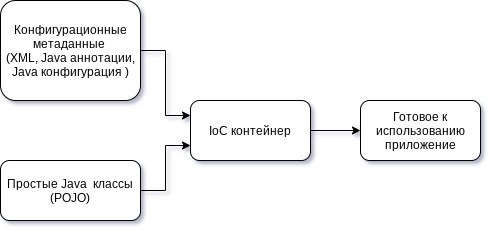
\includegraphics{001_IoC}}
\caption{Упрощенная схема работы IoC контейнера}
\label{fig:image1}
\end{figure}

В данном работе представлен смешанный подход к конфигурации контейнера.

\subsubsection{Spring Boot}

Модуль Spring Boot позволяет наиболее простым и быстрым способом создать веб-приложение, требуя от разработчика минимум усилий по настройке и написанию кода.

Этот модуль обладает большим функционалом, в который входят управление зависимостями,  автоматическая конфигурация и встроенные контейнеры сервлетов для удобного и быстрого тестирования разрабатываемого приложения.

Spring Boot предоставляет возможность автоматической конфигурации приложения, для чего нужно выбрать определенные стартовые пакеты. Ниже представлен фрагмент конфигурационного XML-файла системы сборки Maven, использующейся в дипломном проекте.
\hfill\break
\lstset{language=XML,
basicstyle=\small\sffamily,
numbers=left,
numberstyle=\small,
stepnumber=1,
numbersep=10pt,
showspaces=false,
showstringspaces=false,
showtabs=false,
frame=single,
tabsize=2,
captionpos=b,
breaklines=true,
breakatwhitespace=false,
escapeinside={\%*}{*)} 
}         
\begin{lstlisting}[label=lis1,caption=Зависимости Maven]                
<dependencies>
    <dependency>
        <groupId>org.springframework.boot</groupId>
        <artifactId>spring-boot-starter-web</artifactId>
    </dependency>
    <dependency>
        <groupId>org.springframework.boot</groupId>
        <artifactId>spring-boot-starter-freemarker</artifactId>
    </dependency>
    <dependency>
        <groupId>org.springframework.boot</groupId>
        <artifactId>spring-boot-devtools</artifactId>
        <optional>true</optional>
    </dependency>

    <!-- DataBase support -->
    <dependency>
        <groupId>org.springframework.boot</groupId>
        <artifactId>spring-boot-starter-data-jpa</artifactId>
    </dependency>
    <dependency>
        <groupId>mysql</groupId>
        <artifactId>mysql-connector-java</artifactId>
        <version>8.0.21</version>
        <scope>runtime</scope>
    </dependency>

    <dependency>
        <groupId>org.springframework.boot</groupId>
        <artifactId>spring-boot-starter-security</artifactId>
    </dependency>
    <dependency>
        <groupId>org.springframework.security</groupId>
        <artifactId>spring-security-test</artifactId>
        <scope>test</scope>
    </dependency>
</dependencies>
\end{lstlisting}    

\subsubsection{Spring Data}   

Spring Data - модуль Spring, отвечающий за взаимодействие с сущностями базы данных, их организацию, чтение и запись.

Для пользователя работа с базой данных является достаточно прозрачной - нужно создать классы-сущности, остальное модуль Spring сделает сам. Определенные параметры, такие как название столбца или название таблицы в БД, можно указать при помощи соответствующих аннотаций. 

Ниже представлен пример сущности <<Выбор пользователя>>.
\hfill\break
\lstset{language=Java,
basicstyle=\small\sffamily,
numbers=left,
numberstyle=\small,
stepnumber=1,
numbersep=10pt,
showspaces=false,
showstringspaces=false,
showtabs=false,
frame=single,
tabsize=2,
captionpos=b,
breaklines=true,
breakatwhitespace=false,
escapeinside={\%*}{*)} 
}         
\begin{lstlisting}[label=lis2,caption=Пример сущности <<Выбор пользователя>>] 
@Entity
@Table(name = "user_choices")
public class UserChoice {
    @Id
    @GeneratedValue(strategy= GenerationType.AUTO)
    private Long id;

    @ManyToOne(fetch = FetchType.EAGER)
    @JoinColumn(name = "user_id")
    private User user;

    @ManyToOne(fetch = FetchType.EAGER)
    @JoinColumn(name = "dinner_id")
    private Dinner dinner;

    private LocalDate date;
\end{lstlisting}

В предсавленном примере задействованы следующие аннотации для настройки работы Spring Data:

\begin{itemize}
\setlength{\itemsep}{-2mm}
	\item \textbf{@Entity} - указывает, что данный класс является сущностью БД и должен быть в ней сохранен
	\item \textbf{@Table} - описывает таблицу, в которой должна быть сохранена сущность. В круглых скобках указаны параметры, в данном случае параметр name - имя таблицы
	\item \textbf{@Id} - говорит, что это поле является первичным ключом
	\item \textbf{@GeneratedValue} - говорит, что поле @Id должно быть заполнено автоматически
	\item \textbf{@ManyToOne} - указывает на связь "многие к одному"
	\item \textbf{@JoinColumn} - указывает, по какому столбцу осуществляется свять между сущностями
\end{itemize}

Для осуществления взамодействия с БД необходим также репозиторий, наследующий сущность Spring CrudRepository.
\hfill\break
\lstset{language=Java,
basicstyle=\small\sffamily,
numbers=left,
numberstyle=\small,
stepnumber=1,
numbersep=10pt,
showspaces=false,
showstringspaces=false,
showtabs=false,
frame=single,
tabsize=2,
captionpos=b,
breaklines=true,
breakatwhitespace=false,
escapeinside={\%*}{*)} 
}         
\begin{lstlisting}[label=lis3,caption=Репозиторий сущностей <<Выбор пользователя>>] 
public interface UserChoiceRepo extends CrudRepository<UserChoice, Long> {
    Optional<UserChoice> findById(Long id);
    ArrayList<UserChoice> findByDate(LocalDate date);
    ArrayList<UserChoice> findByDateAndUser(LocalDate date, User user);
}
\end{lstlisting}

Spring Data также позволяет легко организовать поиск в БД. Для этого он предлагает создать методы в репозитории, основанные на полях класса сущности, хранимой в нем. Например, для поиска выбора пользователя по дате был реализован метод \textbf{ArrayList<UserChoice> findByDate(LocalDate date)}, возвращающий ArrayList с найденными сущностями. При создании нужно обратить внимание на наименование полей класса сущности - в классе UserChoice есть поле Data, по имени которого и осуществляется генерация метода поиска.

\subsection{Выбор и подключение базы данных}
\subsubsection{Выбор базы данных}

Для хранения информации в проекте использована база данных MySQL. Это свободная реляционная система управления базами данных, разработку и поддержку которой осуществялет корпорация Oracle. 
MySQL имеет ряд преимуществ:

\begin{itemize}
\setlength{\itemsep}{-2mm}
	\item Простота использования. В большинстве дистрибутивов Linux она доступна в базовых репозиториях и устанавливается одной командой в терминале. Для других систем существуют установщики, доступные на официальном сайте, в результате работы которых система так же быстро устанавливается;
	\item Большие возможности для работы с БД;
	\item Безопасность. Система изначально создана таким образом, что множество
встроенных функций безопасности в ней работают по умолчанию. Например, в последних версиях по умолчанию вклюена усиленая проверка паролей, что не позволит создать простой пароль для доступа к БД;
	\item Масштабируемость. Система может быть использована как для малых, так и для больших объемов данных, что подтверждается довольно широким ее распространением в интернет-технологиях и особенно в сайтостроении;
	\item Скорость работы.
\end{itemize}

\subsubsection{Подключение MySQL к проекту}

Для подключения БД к приложению нужно указать соответствующую зависимость в конфигурационном файле системы сборки Maven.
\hfill\break
\lstset{language=XML,
basicstyle=\small\sffamily,
numbers=left,
numberstyle=\small,
stepnumber=1,
numbersep=10pt,
showspaces=false,
showstringspaces=false,
showtabs=false,
frame=single,
tabsize=2,
captionpos=b,
breaklines=true,
breakatwhitespace=false,
escapeinside={\%*}{*)} 
}         
\begin{lstlisting}[label=lis4,caption=Подключение MySQL в Maven>>] 
		<dependency>
            <groupId>org.springframework.boot</groupId>
            <artifactId>spring-boot-starter-data-jpa</artifactId>
        </dependency>
        <dependency>
            <groupId>mysql</groupId>
            <artifactId>mysql-connector-java</artifactId>
            <version>8.0.21</version>
            <scope>runtime</scope>
        </dependency>
\end{lstlisting}

А также указать настройки подключения к БД в файле \textbf{application.properties}:
\hfill\break
\lstset{
basicstyle=\small\sffamily,
numbers=left,
numberstyle=\small,
stepnumber=1,
numbersep=10pt,
showspaces=false,
showstringspaces=false,
showtabs=false,
frame=single,
tabsize=2,
captionpos=b,
breaklines=true,
breakatwhitespace=false,
escapeinside={\%*}{*)} 
}         
\begin{lstlisting}[label=lis5,caption=Настройки MySQL в application.properties>>] 
spring.datasource.url=jdbc:mysql://localhost:3306/foodchecker?useUnicode=true&useJDBCCompliantTimezoneShift=true&useLegacyDatetimeCode=false&serverTimezone=UTC
spring.datasource.username=******
spring.datasource.password=********
\end{lstlisting}

И указать настройки, необходимые модулю Spring JPA:
\hfill\break
\lstset{language=XML,
basicstyle=\small\sffamily,
numbers=left,
numberstyle=\small,
stepnumber=1,
numbersep=10pt,
showspaces=false,
showstringspaces=false,
showtabs=false,
frame=single,
tabsize=2,
captionpos=b,
breaklines=true,
breakatwhitespace=false,
escapeinside={\%*}{*)} 
}         
\begin{lstlisting}[label=lis6,caption=Настройки Spring JPA в application.properties>>] 
spring.jpa.hibernate.ddl-auto=update
\end{lstlisting}

\subsection{Spring Web}

Spring Web (включая Spring MVC) – модуль фреймворка Spring, который обеспечивает архитектуру паттерна Model - View - Controller (Модель - Отображение - Контроллер) при помощи слабо связанных готовых компонентов. Паттерн MVC разделяет аспекты приложения (логику ввода, бизнес-логику и логику UI), обеспечивая при этом свободную связь между ними.

\begin{itemize}
\setlength{\itemsep}{-2mm}
	\item\textbf{Model} (Модель) объединяет данные приложения;
	\item\textbf{View} (Отображение, Вид) отвечает за отображение данных Модели — как правило, генерируя HTML код страницы
	\item\textbf{Controller} (Контроллер) обрабатывает запросы пользователя, генерирует данные для модели, формирует модель и передает ее в отображение
\end{itemize}

Логика работы Spring MVC построена вокруг DispatcherServlet, который принимает
и обрабатывает все HTTP-запросы и ответы на них, а именно:

\begin{enumerate}
\setlength{\itemsep}{-2mm}
	\item При получении запроса DispatcherServlet обращается к интерфейсу HandlerMapping, который определяет, какой Контроллер должен быть вызван, после чего, отправляет запрос в нужный Контроллер;
	\item Контроллер принимает переданный ему запрос и вызывает соответствующий служебный метод,основанный на методах GET или POST. Вызванный метод определяет данные Модели, основанные на заложенной разработчиком бизнес-логике, и возвращает в DispatcherServlet имя Вида (View);
	\item При помощи интерфейса ViewResolver DispatcherServlet определяет, какой Вид нужно использовать на основании полученного имени;
	\item После того, как Вид (View) создан, DispatcherServlet отправляет данные Модели в виде атрибутов в Вид, который в итоге отображается в браузере, располагаясь в отведенных им местах;
\end{enumerate}

С точки зрения разработчика центральным узловым элементом приложения, отвечающим за обработку приходящих данных, является \textbf{@Controller}. Ниже приведен пример одного из контроллеров разработанного приложения.
\hfill\break
\lstset{language=Java,
basicstyle=\small\sffamily,
numbers=left,
numberstyle=\small,
stepnumber=1,
numbersep=10pt,
showspaces=false,
showstringspaces=false,
showtabs=false,
frame=single,
tabsize=2,
captionpos=b,
breaklines=true,
breakatwhitespace=false,
escapeinside={\%*}{*)} 
}         
\begin{lstlisting}[label=lis7,caption=@Controller] 
@Controller
public class DinnerControler {
    @Autowired
    private DinnerRepo dinnerRepo;

    @GetMapping("/admin/dinners")
    public String dinners(Model model) {
        Iterable<Dinner> dinners = dinnerRepo.findAll();
        model.addAttribute("dinners", dinners);
        return "dinners";
    }
}
\end{lstlisting}

В данном контроллере реализованы следующие аннотации:

\begin{itemize}
\setlength{\itemsep}{-2mm}
	\item\textbf{@Controller} сообщает, что данный класс является контроллером;
	\item\textbf{@Autowired} подключает репозиторий для работы с базой данных;
	\item\textbf{@GetMapping} объявляет метод, перехватывающий запрос методом GET по адресу \textbf{/admin/dinners}, получающий из репозитория список существущих в нем обедов и возвращающий страницу <<dinners>> из созданных шаблонов отображения;
\end{itemize}

\subsection{Spring Security}

Spring Security - модуль Spring, организующий механизмы аутентификации и авторизации пользователей, а также другие связанные с ними возможности обеспечения безопасности Java-приложения.

Для включения данных методов необходимо создать унаследованный от WebSecurityConfigurerAdapter класс и переопределить в нем метод конфигурации, задав аннотации \textbf{@Configuration} и \textbf{@EnableWebSecurity}. Ниже показан пример конфигурации безопасности для данной дипломной работы.
\hfill\break
\lstset{language=Java,
	basicstyle=\small\sffamily,
	numbers=left,
	numberstyle=\small,
	stepnumber=1,
	numbersep=10pt,
	showspaces=false,
	showstringspaces=false,
	showtabs=false,
	frame=single,
	tabsize=2,
	captionpos=b,
	breaklines=true,
	breakatwhitespace=false,
	escapeinside={\%*}{*)} 
}         
\begin{lstlisting}[label=lis8,caption=Класс настроек безопасности] 
@Configuration
@EnableWebSecurity
@EnableGlobalMethodSecurity(prePostEnabled = true)
public class WebSecurityConfig extends WebSecurityConfigurerAdapter {
    @Autowired
    private UserService userService;
    @Override
    protected void configure(HttpSecurity http) throws Exception {
        http.httpBasic().disable()
                .authorizeRequests()
                    .antMatchers("/", "/static/**").permitAll()
                    .anyRequest().authenticated()
                .and()
                    .formLogin()
                    .loginPage("/login")
                    .permitAll()
                .and()
                    .logout()
                    .logoutSuccessUrl("/")
                    .clearAuthentication(true)
                    .invalidateHttpSession(true)
                    .permitAll();
    }

    @Override
    protected void configure(AuthenticationManagerBuilder auth) throws Exception {
        auth.userDetailsService(userService)
                .passwordEncoder(NoOpPasswordEncoder.getInstance());
    }
}
\end{lstlisting}


Из приведенного выше класса видно, что доступ неавторизованным пользователям разрешен только к директории со статическим контентом (/static/**) и главной странице (/). Доступ к остальным страницам запрещен.

\subsection{Шаблонизатор FreeMaker}

FreeMarker — компилирующий обработчик шаблонов, написанный на Java, один из инструментов, позволяющих отделить логику и данные от представления в духе концепции Model - View - Controller. Используется преимущественно при разработке web-приложений с использованием Java-сервлетов, также может использоваться для вывода текста в других случаях: генерация CSS, исходного кода Java и т. д. В отличие от JSP FreeMarker не является зависимым от архитектуры сервлета или от протокола HTTP. Таким образом шаблонизатор может использоваться не только в web-проектах. FreeMarker является свободным ПО.

FreeMaker принимает переданную ему Модель (Model) и может как просто вывести ее содержимое в нужных местах, так и обработать: например, проверить наличие чего-либо в переменных, сравнить результаты и так далее. Также он поддерживает разбиение шаблона на части, что применяется в местах, где код одинаковый. Например, каркас основной HTML-страницы лежит в отдельном файла \textbf{*.ftl} и представляет собой следующее:
\hfill\break
\lstset{language=html,
	basicstyle=\small\sffamily,
	numbers=left,
	numberstyle=\small,
	stepnumber=1,
	numbersep=10pt,
	showspaces=false,
	showstringspaces=false,
	showtabs=false,
	frame=single,
	tabsize=2,
	captionpos=b,
	breaklines=true,
	breakatwhitespace=false,
	escapeinside={\%*}{*)} 
}         
\begin{lstlisting}[label=lis9,caption=Шаблон основной страницы] 
<#macro page>
    <!DOCTYPE html>
    <html lang="en">
    <head>
        <meta charset="UTF-8">
        <title>Corporate Food Checker</title>
        <link rel="stylesheet" href="/static/style.css">

        <meta name="viewport" content="width=device-width, initial-scale=1, shrink-to-fit=no">

        <!-- Bootstrap CSS -->
        <link rel="stylesheet" href="https://stackpath.bootstrapcdn.com/bootstrap/4.5.2/css/bootstrap.min.css"
              integrity="sha384-JcKb8q3iqJ61gNV9KGb8thSsNjpSL0n8PARn9HuZOnIxN0hoP+VmmDGMN5t9UJ0Z"
              crossorigin="anonymous">
    </head>
    <body>
    <#include "navbar.ftl">
    <div class="container mt-3">
        <#nested>
    </div>
    <!-- Optional JavaScript -->
    <!-- jQuery first, then Popper.js, then Bootstrap JS -->
    <script src="https://code.jquery.com/jquery-3.5.1.slim.min.js"
            integrity="sha384-DfXdz2htPH0lsSSs5nCTpuj/zy4C+OGpamoFVy38MVBnE+IbbVYUew+OrCXaRkfj"
            crossorigin="anonymous"></script>
    <script src="https://cdn.jsdelivr.net/npm/popper.js@1.16.1/dist/umd/popper.min.js"
            integrity="sha384-9/reFTGAW83EW2RDu2S0VKaIzap3H66lZH81PoYlFhbGU+6BZp6G7niu735Sk7lN"
            crossorigin="anonymous"></script>
    <script src="https://stackpath.bootstrapcdn.com/bootstrap/4.5.2/js/bootstrap.min.js"
            integrity="sha384-B4gt1jrGC7Jh4AgTPSdUtOBvfO8shuf57BaghqFfPlYxofvL8/KUEfYiJOMMV+rV"
            crossorigin="anonymous"></script>
    </body>
    </html>
</#macro>
\end{lstlisting}

Код, генерируемый другими классами приложения будет помещаться вместо тега \textbf{<\#nested>}. Ниже приведен пример использования каркаса на странице выводов списка обедов.
\hfill\break
\lstset{language=html,
	basicstyle=\small\sffamily,
	numbers=left,
	numberstyle=\small,
	stepnumber=1,
	numbersep=10pt,
	showspaces=false,
	showstringspaces=false,
	showtabs=false,
	frame=single,
	tabsize=2,
	captionpos=b,
	breaklines=true,
	breakatwhitespace=false,
	escapeinside={\%*}{*)} 
}         
\begin{lstlisting}[label=lis10,caption=Вывод кода в созданном шаблоне] 
<#import "parts/common.ftl" as common>
<@common.page>
    some code
</@common.page>
\end{lstlisting}

\subsection{Bootstrap}

Bootstrap - свободный набор инструментов для создания сайтов и веб-приложений. Включает в себя HTML- и CSS-шаблоны оформления для типографики, веб-форм, кнопок, меток, блоков навигации и прочих компонентов веб-интерфейса, включая JavaScript-расширения.

В данной дипломной работе весь пользовательский интерфейс основан на компонентах Bootstrap. 

Подключение библиотеки Bootstrap к HTML-странице осуществляется путем добавления ссылки в тег <link>:
\hfill\break
\lstset{language=html,
	basicstyle=\small\sffamily,
	numbers=left,
	numberstyle=\small,
	stepnumber=1,
	numbersep=10pt,
	showspaces=false,
	showstringspaces=false,
	showtabs=false,
	frame=single,
	tabsize=2,
	captionpos=b,
	breaklines=true,
	breakatwhitespace=false,
	escapeinside={\%*}{*)} 
}         
\begin{lstlisting}[label=lis11,caption=Подключение Bootstrap к проекту] 
	<link rel="stylesheet" href="https://stackpath.bootstrapcdn.com/bootstrap/4.5.2/css/bootstrap.min.css"
	integrity="sha384-JcKb8q3iqJ61gNV9KGb8thSsNjpSL0n8PARn9HuZOnIxN0hoP+VmmDGMN5t9UJ0Z"
	crossorigin="anonymous">
\end{lstlisting}

\section{Функции системы}

\subsection{Аутентификация в системе}

В начальном состоянии системы существует только один пользователь - <<Администратор>>, логин которого (admin) потом можно изменить в настройках пользователей. Регистрации новых пользователей не существует, учетные записи для каждого пользователя создает администратор в административной панели приложения.

Не аутентифицированному пользователю доступна только главная страница приложения. 

\begin{figure}[h]
\center{
\includegraphics[width=1\linewidth]{002}}
\caption{Главная страница приложения}
\label{fig:image2}
\end{figure}

На белом поле ниже полосы главного меню в будущем будут отображаться новости проекта и предприятия.

При попытке доступа к другим страницам пользователю будет показана страница входа, также доступная по нажатию кнопки <<Вход>> в правом верхнем углу страницы.

\begin{figure}[h]
\center{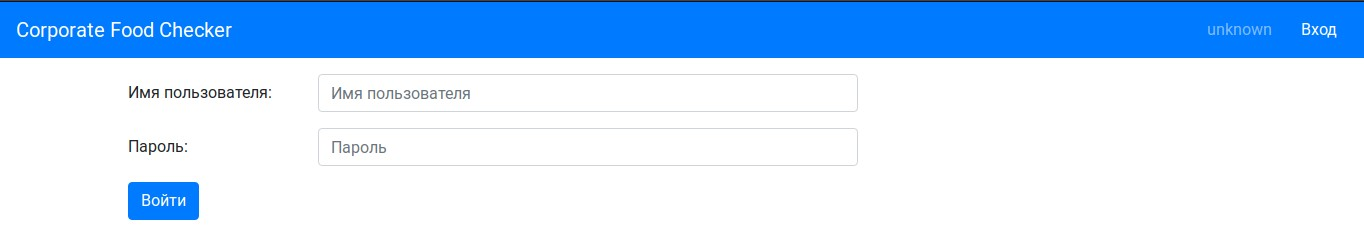
\includegraphics[width=1\linewidth]{003}}
\caption{Страница входа}
\label{fig:image3}
\end{figure}

После успешного логина в зависимости от роли пользователя ему будет показаны дополнительные пункты меню вверху страницы. Всего ролей пользователей существует две:

\begin{itemize}
\setlength{\itemsep}{-2mm}
	\item\textbf{Пользователь (User)} - имеет доступ только к странице выбора обеда на ближайшие четырнадцать дней;
	\item\textbf{Администратор (Admin)} - имеет доступ к настройкам новых обедов, установкам их на даты, а также к созданию и удалению новых пользователей.
\end{itemize}

Для выхода из системы предусмотрена кнопка <<Выход>> в правом верхнем углу страницы. Слева от нее показано имя текущего пользователя (его логин).

\begin{figure}[h]
\center{
\includegraphics{004}}
\caption{Кнопка выхода из системы}
\label{fig:image4}
\end{figure}

\subsection{Панель администратора}

\subsubsection{Алгоритм работы с приложением}

Для правильного функционирования администратор приложения должен следовать определенному алгоритму действий:

\begin{enumerate}
\setlength{\itemsep}{-2mm}
	\item (\textit{Опционально}) Создать учетные записи пользователей либо проверить их на соответствие реальности. 
	\item Создать доступные для выбора варианты обедов.
	\item Назначить созданные варианты обедов соответствующим датам на ближайшие 14 дней.
\end{enumerate}

\subsubsection{Создание и удаление учетных записей}

Добавление и администрирование учетных записей пользователей осуществляется на странице \textbf{<<Список пользователей>>}.

На ней в виде таблицы отображаются все существующие учетные данные пользователей в виде таблицы (рисунок ~\ref{fig:image5}). 

Для каждого пользователя в таблице отображаются следующие данные:

\begin{itemize}
\setlength{\itemsep}{-2mm}
	\item \textbf{Имя пользователя} - имя пользователя, оно же логин для входа в систему;
	\item \textbf{Права} - права пользователя в системе;
	\item \textbf{Функции} - действия, доступные для произведения с учетной записью;  
\end{itemize}

\begin{figure}[h]
\center{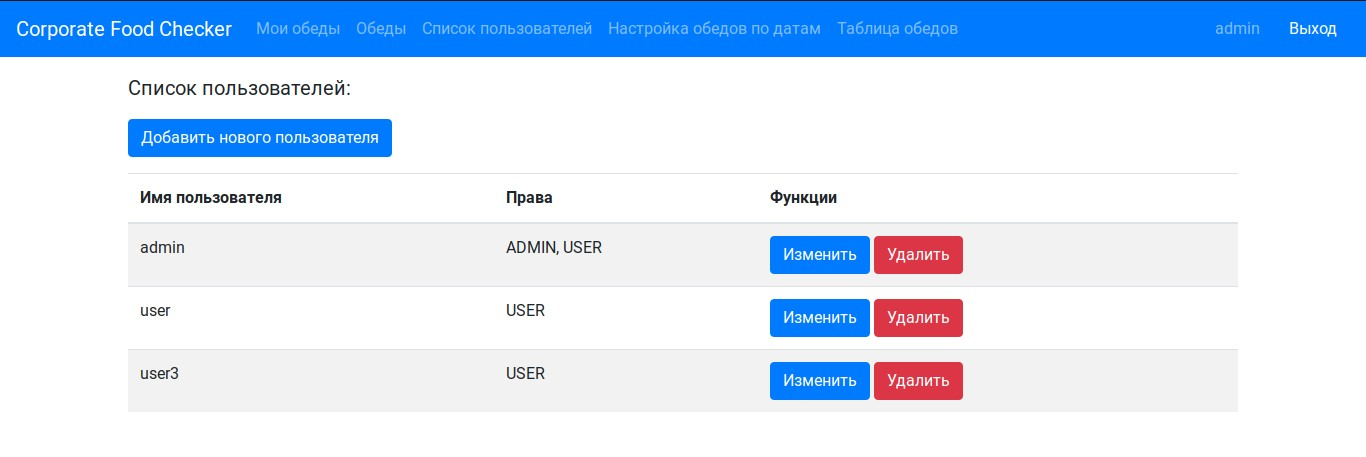
\includegraphics[width=1\linewidth]{005}}
\caption{Страница списка пользователей}
\label{fig:image5}
\end{figure}

Для добавления нового пользователя необходимо нажать на кнопку \textbf{<<Добавить нового пользователя>>} и в появившейся форме ввести данные - имя пользователя и пароль (рисунок ~\ref{fig:image6}).

\begin{figure}[h]
\center{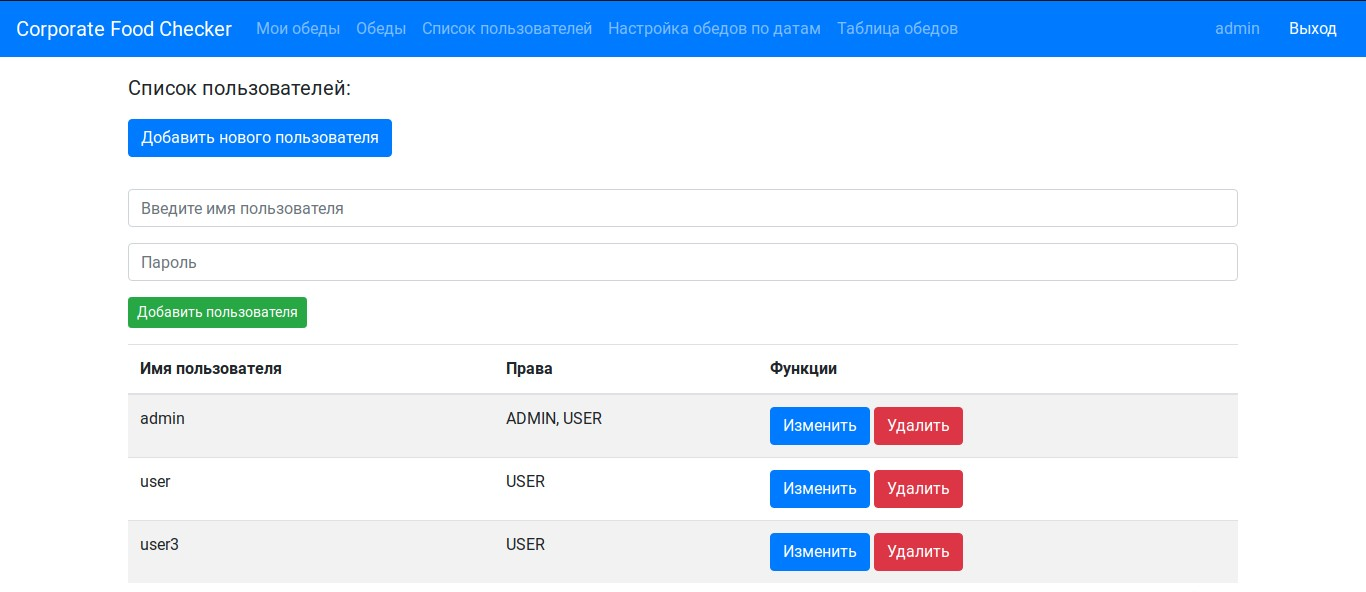
\includegraphics[width=1\linewidth]{006}}
\caption{Форма добавления нового пользователя}
\label{fig:image6}
\end{figure}

По нажатию кнопки \textbf{<<Добавить>>} пользователь будет добавлен, после чего произойдет редирект на страницу пользователей (рисунок ~\ref{fig:image7}). 

\begin{figure}[h]
\center{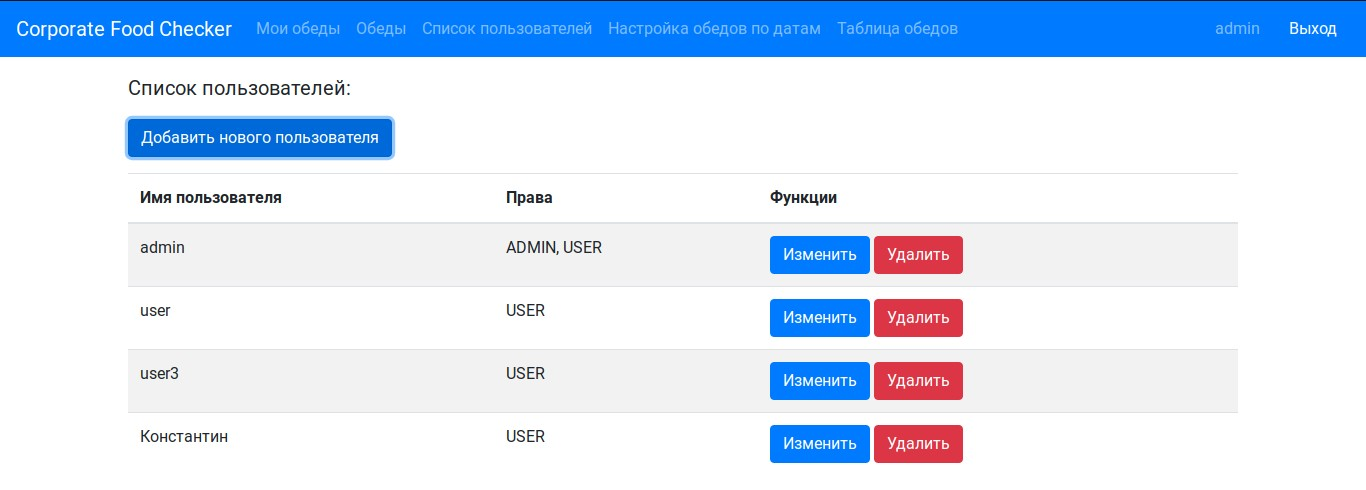
\includegraphics[width=1\linewidth]{007}}
\caption{Форма пользователей с только что созданным пользователем}
\label{fig:image7}
\end{figure}

По умолчанию новый пользователь имеет права \textbf{<<User>>}. Для добавления его в группу администраторов (при необходимости), а также для изменения его имени или пароля необходимо нажать на кнопку \textbf{<<Изменить>>}, расположенную справа от каждой записи пользователя (рисунок ~\ref{fig:image6}).

После нажатия на кнопку появится форма изменения учетной записи пользователя (рисунок ~\ref{fig:image8}).

\begin{figure}[h]
\center{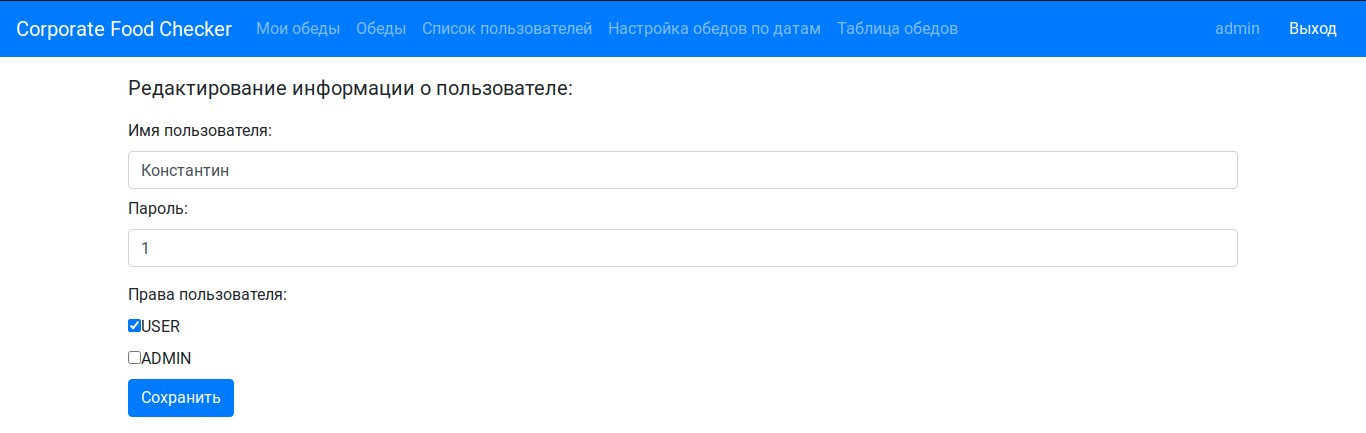
\includegraphics[width=1\linewidth]{008}}
\caption{Форма изменения учетной записи пользователя}
\label{fig:image8}
\end{figure}

Для завершения редактирования необходимо нажать кнопку \textbf{<<Сохранить>>}.

Для удаления учетной записи пользователя необходимо нажать на кнопку \textbf{<<Удалить>>} рядом с кнопкой \textbf{<<Изменить>>} (рисунок ~\ref{fig:image6}). Приложение уточнит, точно ли стоит удалять этого пользователя, и после получения подтверждения удалит его из БД (рисунок ~\ref{fig:image9}).

\begin{figure}[h]
\center{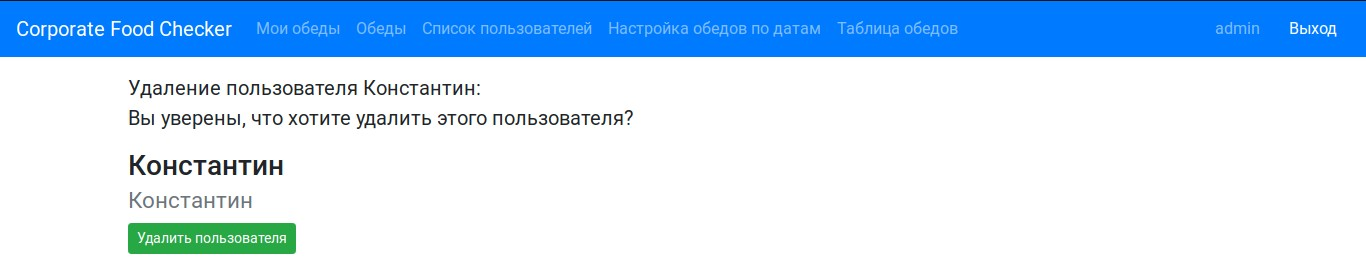
\includegraphics[width=1\linewidth]{009}}
\caption{Подтверждение удаления пользователя}
\label{fig:image9}
\end{figure} 

\subsubsection{Создание вариантов обедов}

Главной задачей приложения является выбор пользователем обеда на текущую дату и на несколько дней вперед. 

Создание вариантов обедов, доступных пользователю для выбора, осуществляется на странице \textbf{<<Обеды>>}. Созданные варианты обедов отображаются в таблице со следующими полями:

\begin{itemize}
\setlength{\itemsep}{-2mm}
	\item \textbf{№} - автоматически генерируемый идентификатор обеда, необходимый для визуального разграничения администратором обедов с одинаковым названием;
	\item \textbf{Название} - название обеда;
	\item \textbf{Описание} - описание обеда, включающее какую-либо информацию по его содержимому;
	\item \textbf{Функции} - действия, доступные для произведения с записью обеда; 
\end{itemize}

На рисунке ~\ref{fig:image10} показан внешний вид страницы обедов. 

\begin{figure}[h]
\center{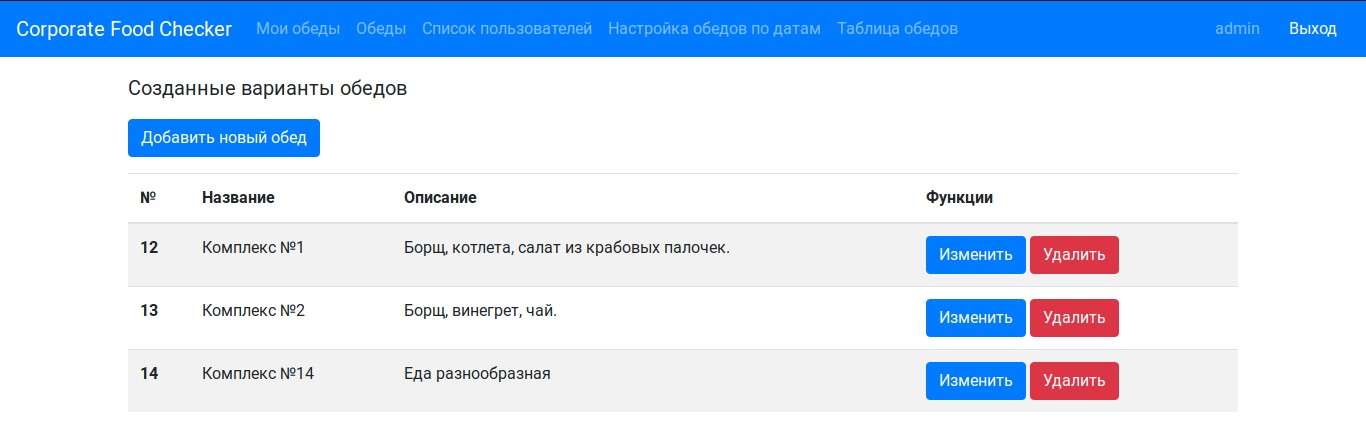
\includegraphics[width=1\linewidth]{010}}
\caption{Страница <<Обеды>>}
\label{fig:image10}
\end{figure}

Для добавления нового обеда необходимо нажать кнопку \textbf{<<Добавить новый обед>>} в верхней части страницы и в открывшейся форме добавления обеда ввести название и описание нового обеда (рисунок ~\ref{fig:image11}).

\begin{figure}[h]
\center{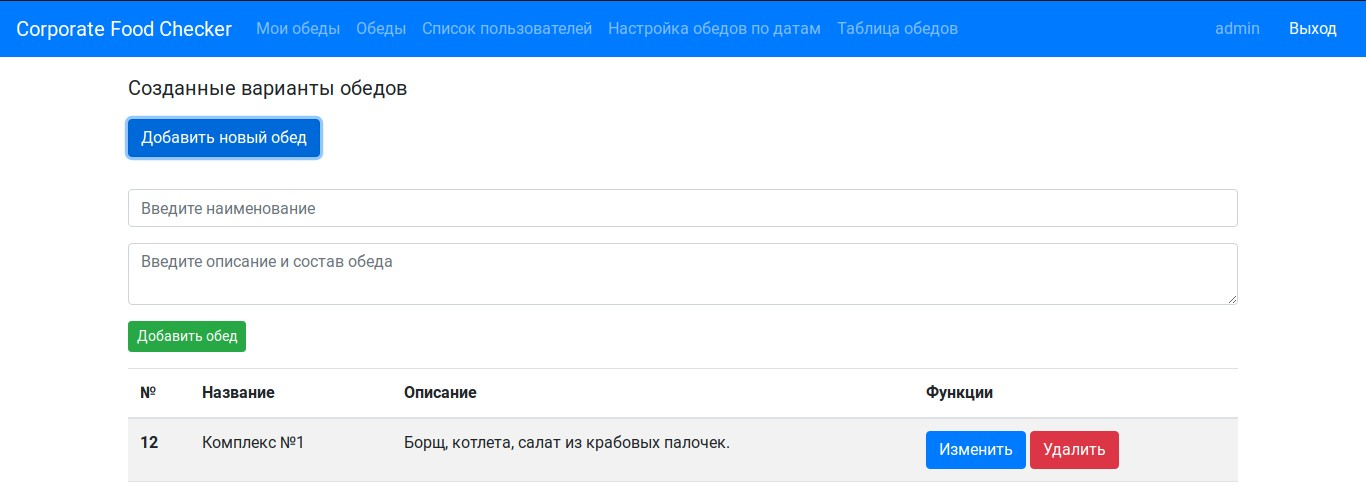
\includegraphics[width=1\linewidth]{011}}
\caption{Форма добавления нового обеда}
\label{fig:image11}
\end{figure}

\subsubsection{Настройка обедов по датам}

После успешного создания вариантов комплексов обедов нужно сопоставить их с датами, начиная с текущей. Сделать это можно на странице \textbf{<<Настройка обедов по датам>>} (рисунок ~\ref{fig:image12}).

\begin{figure}[h]
\center{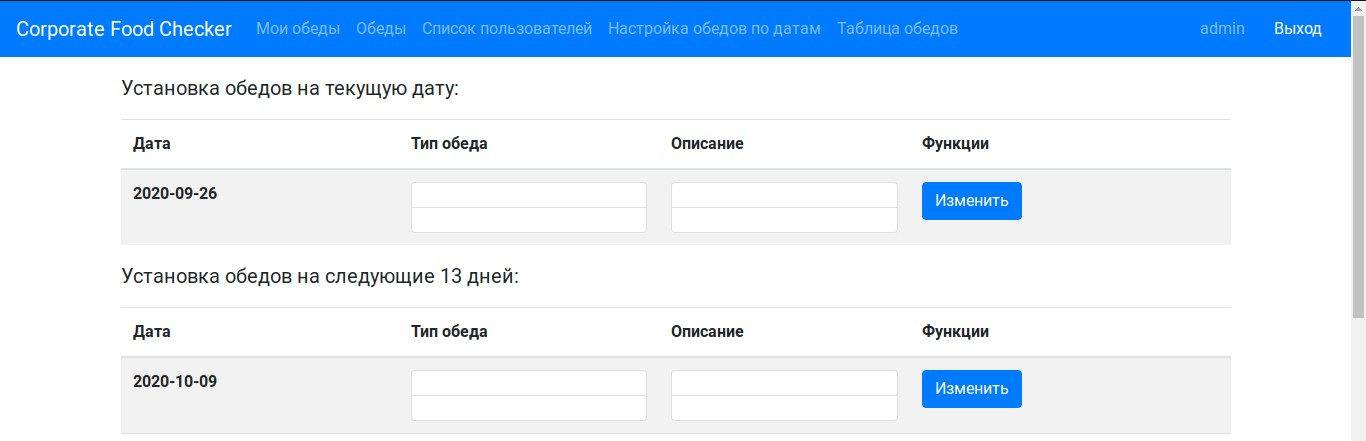
\includegraphics[width=1\linewidth]{012}}
\caption{Страница <<Настройка обедов по датам>>}
\label{fig:image12}
\end{figure}

Отображение сопоставление обедов с датами отображается в виде таблицы со следующими полями:

\begin{itemize}
\setlength{\itemsep}{-2mm}
	\item \textbf{Дата} - дата, на которую устанавливается обед в формате ГГГГ-ММ-ДД;
	\item \textbf{Тип обеда} - в поле представлены два варианта установленных администратором обедов;
	\item \textbf{Описание} - описание обедов, включающее какую-либо информацию по их содержимому;
	\item \textbf{Функции} - доступно лишь одно действие - <<Изменить>>; 
\end{itemize}

Таблица разделена на две - на текущую дату и на тринадцать следующих дней.

Для изменения обеда на дату нужно нажать кнопку \textbf{<<Изменить>>} (рисунок ~\ref{fig:image13}). На открывшейся странице будет доступен выбор из двух вариантов обеда - первый обед и второй обед, каждый из которых можно установить из заранее созданных обедов в разделе <<Создание вариантов обедов>>.

После выбора обедов необходимо нажать кнопку \textbf{<<Сохранить>>} для записи выбора в БД. После сохранение произойдет редирект обратно на страницу настроек обедов по датам (рисунок ~\ref{fig:image14}).

\begin{figure}[h]
\center{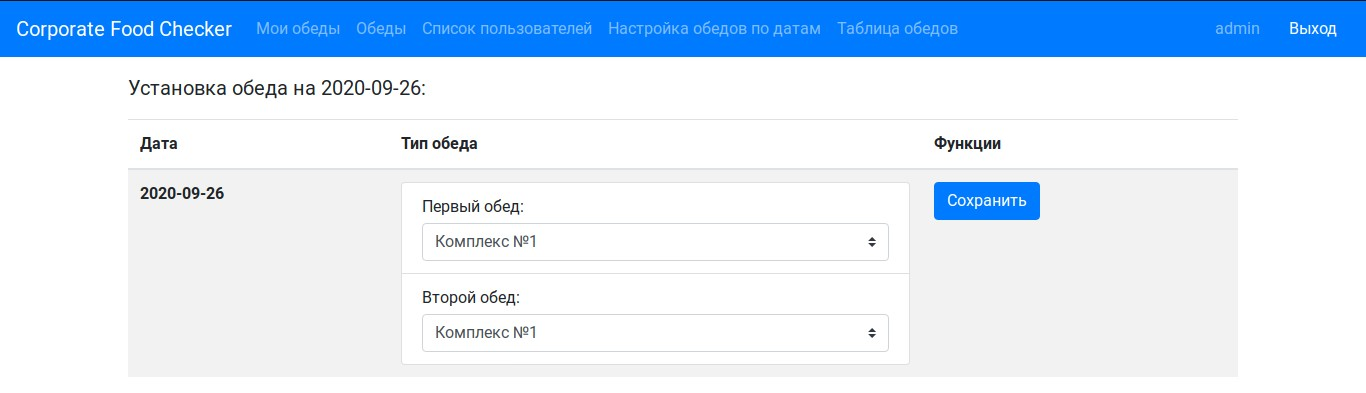
\includegraphics[width=1\linewidth]{013}}
\caption{Страница установки обеда на дату}
\label{fig:image13}
\end{figure}

\begin{figure}[h]
\center{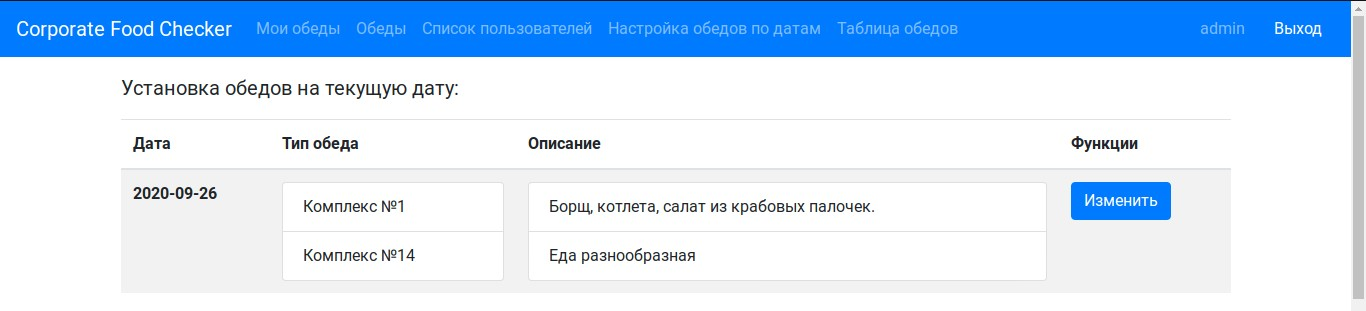
\includegraphics[width=1\linewidth]{014}}
\caption{Страница установки обеда на дату после изменения обеда}
\label{fig:image14}
\end{figure}


\subsection{Взаимодействие с системой от лица простого пользователя}

Простому пользователю доступен только один вариант взаимодействия с системой - осуществление выбора обеда, который он хотел бы получить в определенную дату, начиная с текущей и на тринадцать дней вперед.

Выбор обедов доступен на странице \textbf{<<Мои обеды>>}, доступ к которой появляется только после авторизации в системе. Администратор системы также имеет к ней доступ как обычный пользователь (рисунок ~\ref{fig:image15}).

\begin{figure}[h]
\center{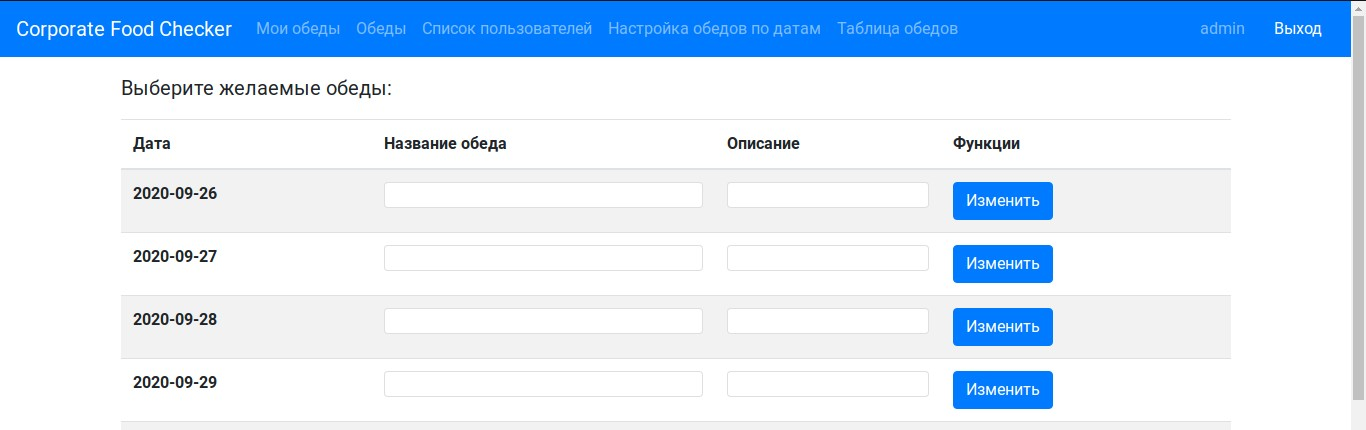
\includegraphics[width=1\linewidth]{015}}
\caption{Страница выбора желаемых обедов пользователем}
\label{fig:image15}
\end{figure}

Выбранные обеды отображаются в виде таблицы со следующими полями:

\begin{itemize}
\setlength{\itemsep}{-2mm}
	\item \textbf{Дата} - дата, на которую выбран обед в формате ГГГГ-ММ-ДД;
	\item \textbf{Название обеда} - название обеда, выбранного на текущую дату;
	\item \textbf{Описание} - описание обеда, включающее какую-либо информацию по его содержимому;
	\item \textbf{Функции} - доступно лишь одно действие - <<Изменить>>; 
\end{itemize}

Для выбора обеда необходимо нажать на кнопку \textbf{<<Изменить>>} в поле функций на нужной строке обеда. На открывшейся странице (рисунок ~\ref{fig:image16}) будет доступен выбор из двух обедов, установленных администратором на эту дату. 

\begin{figure}[h!]
\center{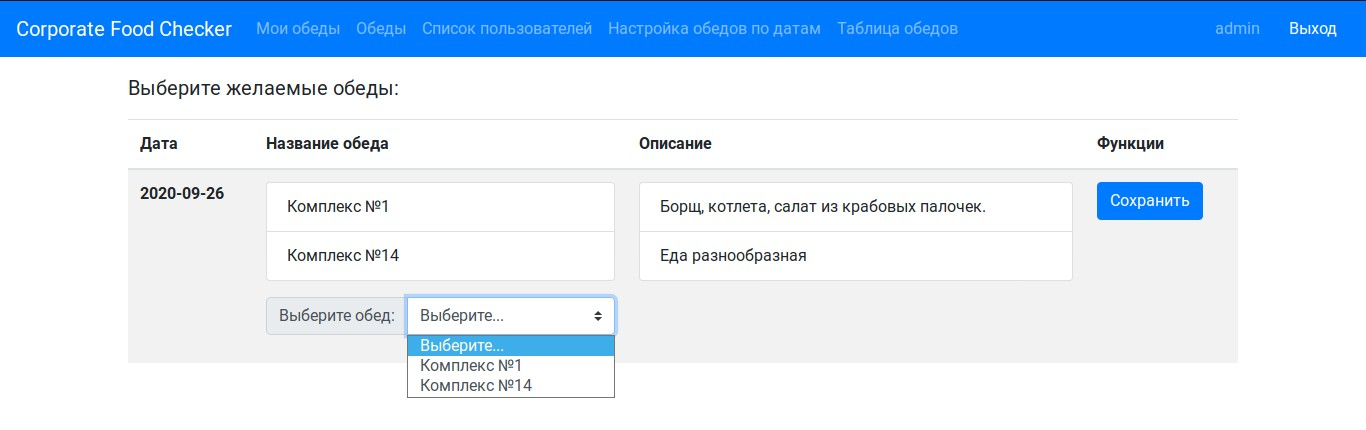
\includegraphics[width=1\linewidth]{016}}
\caption{Страница выбора желаемого обеда на дату}
\label{fig:image16}
\end{figure}

После выбора в выпадающем списке нужного обеда необходимо нажать кнопку <<Сохранить>>, после чего произойдет редирект на страницу <<Мои обеды>> (рисунок ~\ref{fig:image17}).

\begin{figure}[h!]
\center{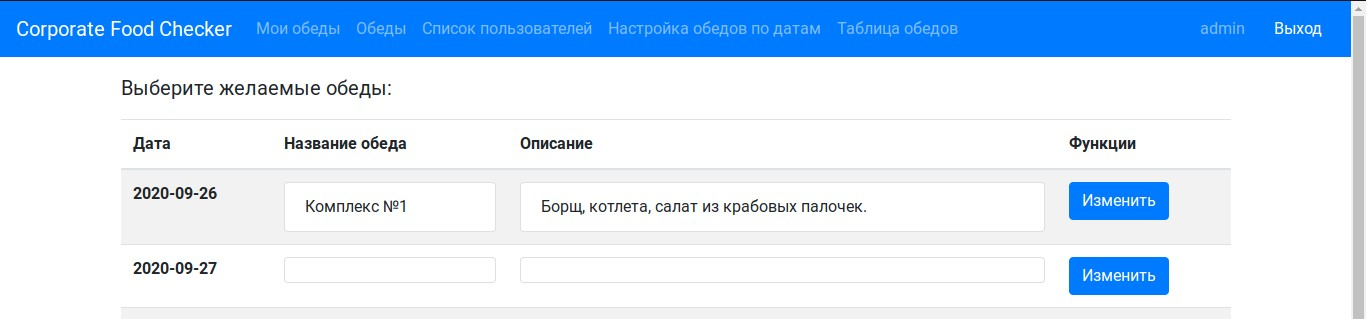
\includegraphics[width=1\linewidth]{017}}
\caption{Страница выбора желаемых обедов пользователем с выбранным обедом}
\label{fig:image17}
\end{figure}

\subsection{Просмотр статистики выбранных обедов}

Просмотреть статистику выбранных пользователями обедов может только администратор приложения. Для этого нужно перейти на страницу \textbf{<<Таблица обедов>>} (рисунок ~\ref{fig:image18}).

\begin{figure}[h]
\center{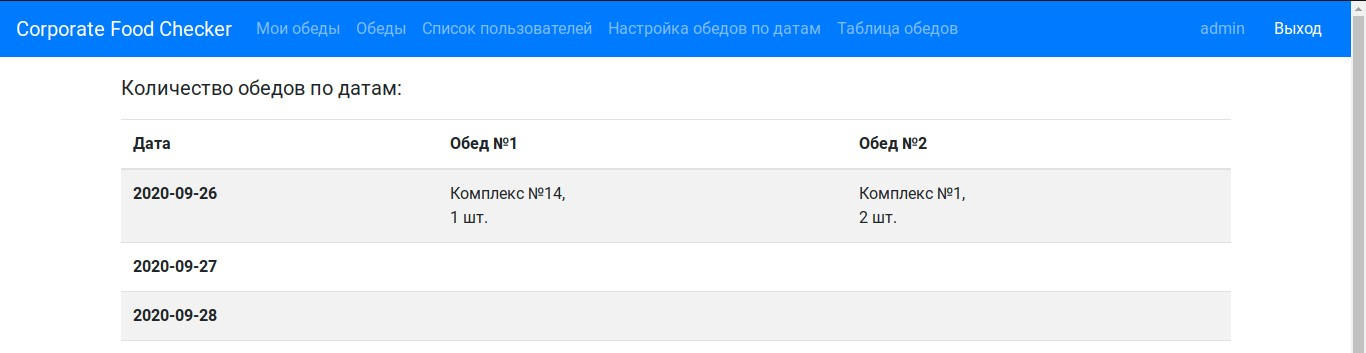
\includegraphics[width=1\linewidth]{018}}
\caption{Страница <<Таблица обедов>>}
\label{fig:image18}
\end{figure}

Количество выбранных пользователями обедов на каждую из дат отображается в виде таблицы, содержащей следующие поля:

\begin{itemize}
\setlength{\itemsep}{-2mm}
	\item \textbf{Дата} - дата, на которую выбраны обеды в формате ГГГГ-ММ-ДД;
	\item \textbf{Обед №1} - название и количество обедов №1;
	\item \textbf{Обед №2} - название и количество обедов №2;
\end{itemize}

\section{Структура данных}

\subsection{Диаграмма базы данных}

На рисунке ~\ref{fig:image19} представлена модель базы данных приложения.

\begin{figure}[h]
\center{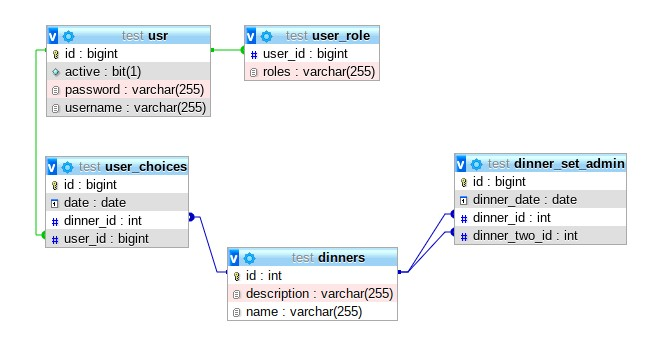
\includegraphics[width=1\linewidth]{019}}
\caption{Модель базы данных}
\label{fig:image19}
\end{figure}

\subsection{Описание сущностей БД}

\begin{enumerate}
\setlength{\itemsep}{-2mm}
	\item \textbf{usr} - пользователь системы;
	\begin{itemize}
	\setlength{\itemsep}{-2mm}
		\item \textbf{id} - уникальный идентификатор пользователя (генерируется автоматически);
		\item \textbf{username} - имя пользователя;
		\item \textbf{password} -  пароль пользователя;
	\end{itemize}
	\item \textbf{user\_role} - роли пользователей;
		\begin{itemize}
		\setlength{\itemsep}{-2mm}
			\item \textbf{user\_id} - идентификатор пользователя (ссылается на ID сущности usr);
			\item \textbf{roles} - роли пользователя;
		\end{itemize}
	\item \textbf{dinners} - варианты обедов;
		\begin{itemize}
			\setlength{\itemsep}{-2mm}
				\item \textbf{id} - уникальный идентификатор обеда (генерируется автоматически);
				\item \textbf{description} - описание обеда;
				\item \textbf{name} -  название обеда;
			\end{itemize}
	\item \textbf{dinner\_set\_admin} - установка обеда на конкретную дату
		\begin{itemize}
			\setlength{\itemsep}{-2mm}
				\item \textbf{id} - уникальный идентификатор установки;
				\item \textbf{dinner\_date} - дата установки;
				\item \textbf{dinner\_id} - идентификатор обеда №1 (ссылается на id обеда сущности dinners);
				\item \textbf{dinner\_two\_id} - идентификатор обеда №2 (ссылается на id обеда сущности dinners);
			\end{itemize}
	\item \textbf{user\_choices} - выбор пользователя на конкретную дату
		\begin{itemize}
					\setlength{\itemsep}{-2mm}
						\item \textbf{id} - уникальный идентификатор выбора пользователя (генерируется автоматически);
						\item \textbf{dinner\_id} - идентификатор обеда (ссылается на id обеда сущности dinners);
						\item \textbf{user\_id} -  идентификатор пользователя (ссылается на id пользователя сущности usr);
					\end{itemize}
\end{enumerate}

\newpage
\section{Заключение}

В ходе выполнения дипломной работы была разработана система выбора обедов пользователями на предприятии.

Изучена теория на тему создания веб-приложений (как сервеной, так и клиентской части), работы с системой контроля версий GIT, изучены некоторые модули фреймворка Spring, необходимые для разработки приложений на языке Java.

Для сборки приложения использована система Maven.

Данное приложение является MVP (минимально жинзеспособным продуктом) и готово к внедрению в компанию, которая выступала в роли заказчика. Доработка проекта будет осуществляться путем добавления нового функционала, улучшения внешнего вида и интерфейса пользователя, а также разработкой мобильного приложения.

\newpage
\addcontentsline{toc}{section}{Список листингов кода}
\lstlistoflistings

\newpage
\addcontentsline{toc}{section}{Список рисунков}
\listoffigures

\newpage
\addcontentsline{toc}{section}{Список литературы}
\begin{thebibliography}{5}
\bibitem{Sulsky1994}
Эккель Б. Философия Java. 4-е полное изд. --- Спб.: Питер, 2015. --- 1168с.: ил.
\bibitem{Vshivkov}
Уоллс К. Spring в действии. --- М.: ДМК Пресс, 2013. --- 752 с.: ил.
\bibitem{LiuLiu}
Раджпут Динеш Spring. Все паттерны проектирования. --- СПб.: Питер, 2019. --- 320 с.: ил.
\bibitem{Spring}
Spring Framework Documentation --- https://spring.io/
\bibitem{Bootstrap}
Bootstrap Documentation --- https://bootstrap-4.ru/
\end{thebibliography}

\end{document}  % КОНЕЦ ДОКУМЕНТА !